\subsection{Multiple Integrals}
\subsubsection{Double Integrals}
By definition, we get
$$\iint_Rf(x,y)dA=\lim_{M,N\to\infty}\sum_{i=1}^M\sum_{j=1}^Nf(x_{ij}^*,y_{ij}^*)\Delta x\Delta y$$
where $dA=dydx$\\
The double integral can be interpreted as volume under the curve $f(x,y)$.\\
We compute the double integral by first integrating with respect to one variable and then the other.\\
A double integral will be computed in either of the following forms:
\begin{align*}
    &\iint_Rf(x,y)=\int_{x=a}^{x=b}\int_{y=y_1(x)}^{y=y_2(x)}f(x,y)dydx\\
    &\iint_Rf(x,y)=\int_{y=a}^{y=b}\int_{x=x_1(y)}^{x=x_2(y)}f(x,y)dxdy
\end{align*}
Ex: Find $\iint_R ydA$ over the region bounded by $x=y$ and $x=2-y^2$
\begin{align*}
    &\text{intersections: }\\
    &y=2-y^2\Ra y^2+y-2=0\Ra (y+2)(y-1)=0\Ra y=1,\ -2\\
    &\iint ydA=\int_{y=-2}^1\int_{x=y}^{x=2-y^2}ydydx=\int_{-2}^1y\brsquare{x}_y^{2-y^2}dy\\
    &=\int_{-2}^1y(2-y^2-y)dy=\int_{-2}^1(2y-y^3-y^2)dy\\
    &=\brsquare{y^2-\frac{y^4}{4}-\frac{y^3}{3}}_{-2}^1=1-\frac{1}{4}-\frac{1}{3}-\brround{4-4+\frac{8}{3}}=-\frac{9}{4}
\end{align*}
Note that the rules for even/odd functions are the same as with single integrals. If you have an odd function over a symmetric region, the entire integral will be zero. If you have an even function over a symmetric region, you can simplify the region and double the integral.\\
Applications of double integrals:\\
Area of a region:
$$\text{Area}(R)=\iint_RdA$$
The average value of a function can be computed as:
$$\overline{f(x,y)}=\frac{1}{\text{Area}(R)}\iint_Rf(x,y)dA$$
Average height of a region:
$$\overline{y}=\frac{1}{\text{Area}(R)}\iint_RydA$$
Surface Area:
$$S=\iint_R\sqrt{1+f_x^2+f_y^2}dA$$
Center of mass:
$$x_{CM}=\frac{1}{\text{Mass}(R)}\iint_R x\rho(x,y)dA$$
Moment of inertia about an axis $a$ where $D(x,y)$ is the distance from the axis.
$$I_a=\iint_R(D(x,y))^2\rho(x,y)dA$$

\subsubsection{Polar Coordinates}
Polar coordinates uses the variables $r$ and $\theta$ to describe functions.\\
$r$ is the distance from the origin\\
$\theta$ is the angle from the x-axis to the line formed by $r$.\\
We can convert between polar coordinates and rectangular coordinates using the following conversions:
\begin{align*}
    &r=\sqrt{x^2+y^2}\\
    &x=r\cos\theta\\
    &y=r\sin\theta
\end{align*}
Some common expressions in polar coordinates are:
\begin{align*}
    &\text{circle: }r=a\\
    &\text{ray: }\theta=a\\
\end{align*}
Ex: Find the equation of an off-center circle in polar coordinates
\begin{align*}
    &(x-a)^2+y^2=a^2\\
    &x^2-2ax+a^2+y^2=a^2\\
    &\text{recall }r^2=x^2+y^2\\
    &\Ra r^2-2ax=0\\
    &r^2-2ar\cos\theta=0\\
    &r^2=2ar\cos\theta\\
    &r=2a\cos\theta
\end{align*}
Graphing in Polar Coordinates:\\
We can create some interesting graphs using polar coordinates. Here are a few examples:\\
Ex1: $r=\sin(2\theta)$\\
\centerline{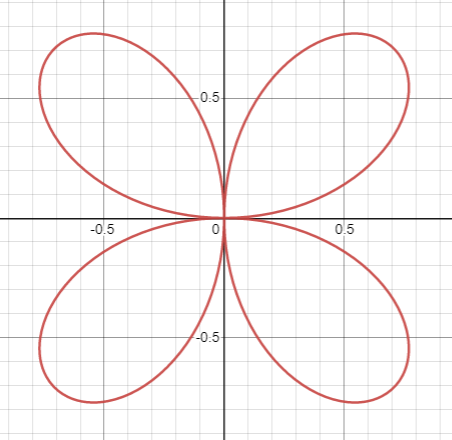
\includegraphics[scale=0.7]{Images/PreCalcPictures/PolarGraph1.png}}
Ex2: $r=1+\cos\brround{\frac{\theta}{2}}$\\
\centerline{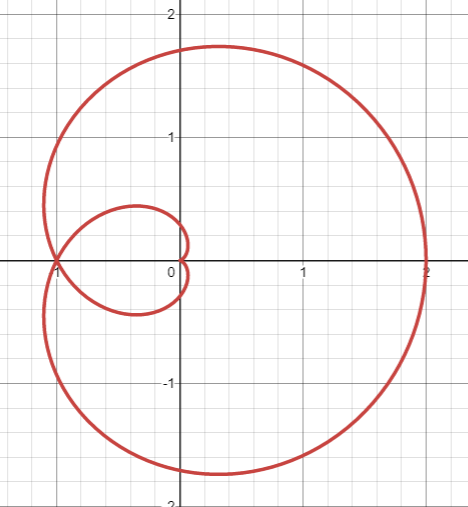
\includegraphics[scale=0.7]{Images/PreCalcPictures/PolarGraph2.png}}

For regions with circular symmetry, it is often easier to integrate in polar coordinates.\\
The differential area is given by:
\begin{align*}
    &dA=rdrd\theta
\end{align*}
Note: This distortion factor of $r$ in $dA=rdrd\theta$ comes from the arc length.\\
Ex: Area of a circle of radius $R$
\begin{align*}
    &\int_{\theta=0}^{\theta=2\pi}\int_{r=0}^{r=R}rdrd\theta\\
    &\int_0^{2\pi}\brsquare{\frac{r^2}{2}}_0^Rd\theta=\int_0^{2\pi}\frac{R^2}{2}d\theta=\pi R^2
\end{align*}
\begin{align*}
    \text{Ex2: }&\int_{-\infty}^\infty e^{-x^2}dx\\
    &\text{let }I=\int_{-\infty}^\infty e^{-x^2}dx,\ I^2=\int_{-\infty}^\infty e^{-x_1^2}dx_1\int_{-\infty}^\infty e^{-x_2^2}dx_2=\int_{x_1=-\infty}^\infty\int_{x_2=-\infty}^\infty e^{-x_1^2}e^{-x_2^2}dx_2dx_1\\
    &I^2=\iint_{\R^2}e^{-x_1^2-x_2^2}dA\\
    &r^2=x_1^2+x_2^2\\
    &I^2=\int_{\theta=0}^{2\pi}\int_{r=0}^\infty e^{-r^2}rdrd\theta=2\pi\int_0^\infty re^{-r^2}dr=2\pi\brsquare{-\frac{e^{-r^2}}{2}}_0^\infty=2\pi\brround{\frac{1}{2}}\\
    &I^2=\pi\\
    &I=\sqrt{\pi}
    \end{align*}
\subsubsection{Triple Integrals}
By definition, we get
$$\iiint f(x,y,z)dV=\lim_{\Delta x,\Delta y,\Delta z\to0}\sum_{i=1}^L\sum_{j=1}^M\sum_{k=1}^Nf(x_{ijk}^*,y_{ijk}^*,z_{ijk}^*)\Delta x\Delta y\Delta z$$
These are computed in the same manner as double integrals, just with an additional step.\\
\begin{align*}
    &\text{Ex: }\iiint_E 2xdV\text{, where $E$ is the region in the first octant bounded by }2x+3y+z=6\\
    &I=\int_{x=0}^3\int_{y=0}^{y=-\frac{2}{3}x+2}\int_{z=0}^{z=6-2x-3y}2xdzdydx\\
    &I=\int_{x=0}^3\int_{y=0}^{y=-\frac{2}{3}x+2}2x(6-2x-3y)dydx\\
    &I=\int_0^3\brsquare{12xy-4x^2y-3xy^2}_{y=0}^{y=-\frac{2}{3}x+2}dx\\
    &I=\int_0^3\brround{\frac{4}{3}x^3-8x^2+12x}dx\\
    &I=9
\end{align*}
Ex2: Find the volume of intersection between the cylinders $x^2+y^2=R^2$ and $x^2+z^2=R^2$
\begin{align*}
    &V=\iiint dV=\int_{x=-R}^R\int_{y=-\sqrt{R^2-x^2}}^{\sqrt{R^2-x^2}}\int_{z=-\sqrt{R^2-x^2}}^{\sqrt{R^2-x^2}}dzdydx\\
    &V=\int_{x=-R}^R\int_{y=-\sqrt{R^2-x^2}}^{\sqrt{R^2-x^2}}2\sqrt{R^2-x^2}dydx\\
    &V=\int_{x=-R}^R4(R^2-x^2)dx\\
    &V=4\brsquare{R^2x-\frac{x^3}{3}}_{-R}^R=8\brround{R^3-\frac{R^3}{3}}=\frac{16R^3}{3}
\end{align*}
\subsubsection{Change of Coordinate Systems}
Two common change of coordinates in triple integrals are cylindrical coordinates and spherical coordinates.\\
Cylindrical coordinates is an extention of polar coordinates where the conversions are as follows:
\begin{align*}
    &r=\sqrt{x^2+y^2}\\
    &x=r\cos\theta\\
    &y=r\sin\theta\\
    &z=z\\
    &dV=rdzdrd\theta
\end{align*}
\centerline{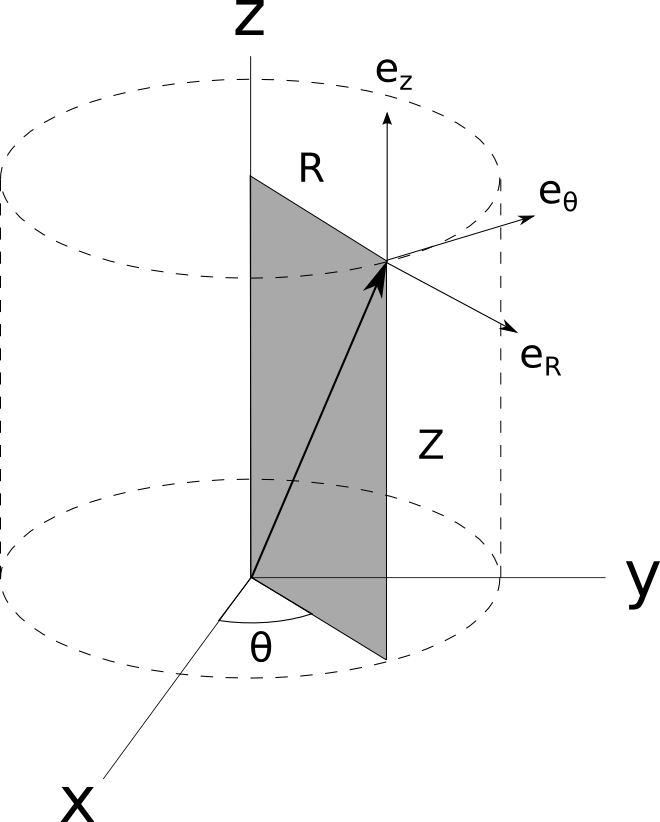
\includegraphics[scale=0.3]{Images/Math217Pictures/cylindricalCoordinates.png}}
Ex: Find the volume of the region below the paraboloid $z=5-x^2-y^2$ and above the plane $z=1$
\begin{align*}
    &\text{Projected area is }\{z=5-x^2-y^2\}\cap\{z=1\}\Ra x^2+y^2=4\\
    &V=\int_{\theta=0}^{2\pi}\int_{r=0}^2\int_{z=1}^{5-r^2}rdzdrd\theta=2\pi\int_0^2 (4r-r^3)dr=2\pi\brsquare{2r^2-\frac{r^4}{4}}_0^2\\
    &V=2\pi\brround{8-4}=8\pi
\end{align*}
Spherical coordinates is given by
\begin{align*}
    &\rho^2=x^2+y^2+z^2\\
    &x=\rho\cos\theta\sin\phi\\
    &y=\rho\sin\theta\sin\phi\\
    &z=\cos\phi\\
    &dV=\rho^2\sin\phi d\rho d\phi d\theta
\end{align*}
\centerline{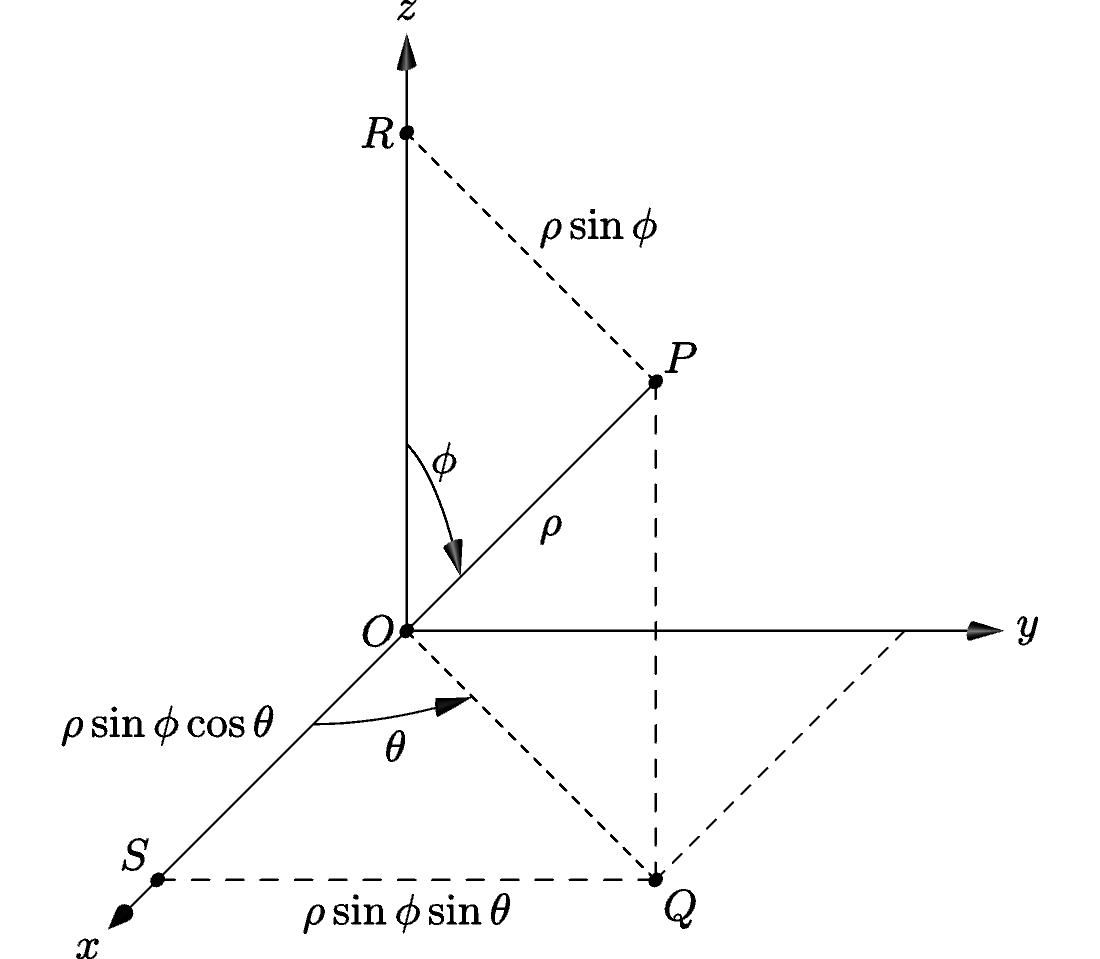
\includegraphics[scale=0.3]{Images/Math217Pictures/sphericalCoordinates.png}}
Ex: Find the volume below the sphere $x^2+y^2+z^2=4$ and above the cone $z=\sqrt{x^2+y^2}$
\begin{align*}
    &V=\int_{\theta=0}^{2\pi}\int_{\phi=0}^{\pi/4}\int_{\rho=0}^2\rho^2\sin\phi d\rho d\phi d\theta=2\pi\int_0^{\pi/4}\frac{8}{3}\sin\phi d\phi=\frac{16\pi}{3}\brsquare{-\cos\phi}_0^{\pi/4}\\
    &V=\frac{16\pi}{3}\brround{1-\frac{1}{\sqrt{2}}}=\frac{8\pi}{3}(2-\sqrt{2})
\end{align*}
We can define an arbitrary change of coordinates in the following way:\\
If we have the equations
$$\eqnsystem{x=x(u,v,w)\\ y=y(u,v,w)\\ z=z(u,v,w)}$$
we can represent the distortion factor as the determinant of the Jacobian.
$$\det J=\detmatrix{x_u&x_v&x_w\\y_u&y_v&y_w\\z_u&z_v&z_w}$$
Ex: Find the volume of the ellipsoid enclosed by the surface $\brround{\frac{x}{a}}^2+\brround{\frac{y}{b}}^2+\brround{\frac{z}{c}}^2=1$
\begin{align*}
    &\text{let }\eqnsystem{x=au\\y=bv\\z=cw}\\
    &\det J=\detmatrix{a&0&0\\0&b&0\\0&0&c}=abc\\
    &V=\iiint_{\brround{\frac{x}{a}}^2+\brround{\frac{y}{b}}^2+\brround{\frac{z}{c}}^2\leq1}dV=\iiint_{u^2+v^2+w^2\leq1}abcdudvdw\\
    &V=abc\cdot\text{Volume(unit sphere)}=\frac{4\pi abc}{3}
\end{align*}